% LaTeX source for ``Algorithms for Computer Simulation of Molecular Systems''
% Copyright (c) 2023 รังสิมันต์ เกษแก้ว (Rangsiman Ketkaew).

% License: Creative Commons Attribution-NonCommercial-NoDerivatives 4.0 International (CC BY-NC-ND 4.0)
% https://creativecommons.org/licenses/by-nc-nd/4.0/

\chapter{การพัฒนาซอฟต์แวร์สำหรับเคมีเชิงคำนวณ}
\label{ch:software_dev}

%----------------------------------------
\section{การเขียนโปรแกรมทางเคมีเชิงคำนวณ}
%----------------------------------------

ถ้าหากผู้อ่านอยากจะศึกษาการเขียนโปรแกรมทางเคมีเชิงคำนวณจะเริ่มยังไงดี เช่น ต้องการเขียนโปรแกรม Density Functional Theory (DFT) 
หรือ Implement วิธีโครงสร้างเชิงอิเล็กทรอนิกส์ (Electronic Structure) ผมขอให้ความเห็นอย่างนี้ครับว่าการจะที่เขียนโปรแกรมทางเคมี%
คำนวณขึ้นมาสักโปรแกรมหนึ่งนั้นใช้เวลามากพอสมควรเพราะว่ามีรายละเอียดที่ซับซ้อนมาก (เวลาที่ใช้ในการเขียนนั้นขึ้นอยู่กับว่าเขียนคนเดียวหรือช่วย%
กันเขียนหลายคน) ดังนั้นผมแนะนำว่าสำหรับผู้ที่เพิ่งเริ่มต้นการเขียนโปรแกรมทางวิทยาศาสตร์ควรศึกษาจากโปรแกรมมาตรฐานที่ได้รับความนิยมอยู่แล้ว 
ผมไม่ได้บอกว่าห้ามเขียนโปรแกรมใหม่เองแบบเริ่มจากศูนย์หรือ From Scratch แต่ถ้าหากว่าเราเริ่มต้นเรียนรู้จากโปรแกรมที่ได้รับความนิยมและใช้งาน%
กันอย่างแพร่หลายอยู่แล้วก็มีข้อดีดังนี้ 

\begin{itemize}
    \item ประหยัดเวลา ไม่ต้องมานั่งศึกษาหรือเขียนโค้ดใหม่เองทั้งหมด
    
    \item ได้เรียนรู้วิธีการเขียนโค้ดที่มีประสิทธิภาพจากนักพัฒนาคนอื่น ๆ 
    
    \item เป็นการต่อยอดและพัฒนาโปรแกรมนั้น ๆ ให้ดีขึ้นไปอีกเพราะเราไม่จำเป็นต้องมา Reinvent the Wheel 
    
    \item เป็นการสร้างเครือข่ายนักวิจัยและความร่วมมือทางวิชาการในระดับนานาชาติ 
\end{itemize}

\noindent อย่างไรก็ตามถ้าหากใครอยากจะเริ่มเขียนโปรแกรมเองนั้น (ไม่จำเป็นต้องเป็น DFT อย่างเดียว แต่รวมถึงวิธีการจำลองทางคอมพิวเตอร์อื่น ๆ 
ด้วย เช่น Molecular Dynamics หรือ Monte Carlo) ก็มีข้อดีหลายข้อเหมือนกัน ดังนี้ 

\begin{itemize}
    \item ได้ทำความเข้าใจการเขียนโปรแกรมอ้างอิงตามสมการทาง Electronic Structure 
    
    \item ฝึกทักษะการเขียนโปรแกรมสำหรับการคำนวณทางวิทยาศาสตร์และได้เรียนรู้เทคนิคการประมาณค่าเชิงตัวเลข
    
    \item ได้ออกแบบโปรแกรมเองและ Implement วิธีใหม่ ๆ ที่โปรแกรมอื่นไม่มี
    
    \item ต่อยอดเป็นโปรแกรมในรูปแบบเชิงพานิชย์ได้เพราะว่ามีโปรแกรมทางเคมีคำนวณหลาย ๆ โปรแกรมที่ขาย License
\end{itemize}

ประเด็นหรือคำถามสำคัญคือ \enquote{ถ้าหากอยากจะเริ่มศึกษาโค้ดของวิธีการคำนวณทางเคมีควอนตัม เช่น โปรแกรม Density Functional 
Theory (DFT) ดี ๆ สักตัวนึงจะเริ่มจากไหนดี?} ความเห็นของผมคือแนะนำให้ศึกษาโปรแกรม PySCF โดยมีเหตุผลดังต่อไปนี้

\begin{itemize}
    \item โปรแกรมมีประสิทธิภาพสูง ทำงานได้เร็วและให้ผลการคำนวณที่ถูกต้องและแม่นยำและยังคำนวณได้หลากหลายวิธี
    
    \item มีผู้ใช้งานเยอะเนื่องจากว่าโปรแกรม PySCF นั้นสามารถติดตั้งและใช้งานได้ง่าย เตรียมไฟล์ Input ได้ไม่ยุ่งยาก 
    
    \item PySCF เขียนด้วย Python เกือบทั้งหมด (87\% เขียนด้วย Python, 12\% เป็นภาษา C ก็คือพวกไลบรารี่ต่าง ๆ ที่เอามาคำนวณ%
    ในส่วนที่ Python อาจจะคำนวณได้ช้า) ดังนั้นจึงง่ายต่อการทำความเข้าใจ
    
    \item มีทีมพัฒนาที่ใหญ่และแข็งแกร่ง ได้รับการสนับสนุนฟีเจอร์และแก้ไข Bug อย่างต่อเนื่อง
\end{itemize}
    
\noindent จากข้อ 1 ถ้าหากเราต้องการ Implement วิธีหรือเทคนิคใหม่ ๆ เข้าไปใน PySCF ก็ทำได้ง่ายเพราะว่าเขียนด้วยภาษา Python 
นอกจากนี้โปรแกรมยังสามารถทำงานด้วย GPU ได้ด้วย (มี Plugin พิเศษชื่อว่า gpu2pyscf) ตัวโค้ดถูกเขียนและได้รับการปรับปรุงมาเป็นอย่างดี 
(Well-written) มีการวางโครงสร้างของโปรแกรมที่เรียบร้อย แบ่ง Methods ต่าง ๆ ออกเป็น Module ที่ชัดเจนและมีการจัดวาง Function 
ที่เหมาะสม สำหรับผู้อ่านที่สนใจโปรแกรม PySCF ก็ไปดูได้ที่ \url{https://github.com/pyscf/pyscf}

เมื่อเราเลือกโปรแกรมได้แล้ว ขั้นตอนต่อมาก็คือพยายามทำความเข้าใจทฤษฎีของหัวข้องานวิจัยที่เราต้องการศึกษา พยายามหาว่าเราสามารถพัฒนา%
วิธีนั้น ๆ ได้อย่างไรเพื่อที่จะปรับปรุงให้มีความถูกต้องในการคำนวณมากขึ้นหรือหากรณีที่ทฤษฎีนั้นยังไม่ครอบคลุม ขั้นตอนต่อไปคือหาวิธีการแก้ไข%
ปัญหาหรือ Solution สำหรับการปรับปรุงทฤษฎีนั้นแล้วเขียนออกมาเป็นสมการทางคณิตศาสตร์ที่เราจะนำไป Implement ได้ ขั้นตอนต่อไปก็คือ%
การวางแผนการเขียนโปรแกรมซึ่งสามารถทำได้ด้วยการเขียนโค้ดเทียมหรือ Pseudo Code ก่อนที่เราจะ Implement จริง ๆ โดยเราจะต้องคิดเกี่ยว%
กับการวางโครงสร้างหรือ Structure ของโปรแกรม เช่น แบ่งโปรแกรมออกเป็นโปรแกรมย่อย ๆ หลายส่วน เช่น แบ่งเป็น modules, functions, 
classes, หรือ types โดยเราควรจะต้องคำนึงถึงการพัฒนาโปรแกรมต่อไปในอนาคตด้วยว่าโปรแกรมของเรานั้นสามารถที่จะรองรับฟีเจอร์ใหม่ ๆ 
ที่นักพัฒนาคนอื่น ๆ จะเข้ามาช่วยพัฒนาเพิ่มเติมได้

หลังจากที่เรา Implement เข้าไปในโปรแกรมเสร็จเรียบร้อยแล้วเราควรจะต้องมีการตรวจสอบการทำงานของโปรแกรมหรือฟังก์ชันต่าง ๆ อย่างสม่ำเสมอ%
เพื่อตรวจสอบค่าที่ได้จากคำนวณว่ามีความถูกต้องและมีความสมเหตุสมผลมากน้อยแค่ไหน เมื่อได้ค่าการคำนวณที่ถูกต้องแล้วขั้นตอนสุดท้ายก็คือการ%
ปรับปรุงหรือทำความสะอาดโค้ดให้มีประสิทธิภาพและอ่านได้ง่ายขึ้น ในขั้นตอนนี้เราสามารถเรียนรู้ได้จากการศึกษาโค้ดที่นักพัฒนาคนอื่นเขียนไว้ก็ได้%
ว่าเขาเขียนอย่างไร ใช้วิธีหรือเทคนิคอะไรที่ทำให้โค้ดรันได้เร็วและมีประสิทธิภาพ นอกจากนี้ยังมีสิ่งอื่น ๆ ที่เราควรจะต้องทำด้วย เช่น เขียน Comment 
หรือทำเอกสารประกอบการใช้งาน (Documentation) เพื่อที่ว่าตัวเราเองหรือนักพัฒนาคนอื่น ๆ ที่มาอ่านหรือแก้ไขโค้ดของเรานั้นสามารถทำความ%
เข้าใจโค้ดได้ง่ายและไม่ต้องมานั่งศึกษาเองจากศูนย์

%----------------------------------------
\section{การวางโครงสร้างโปรแกรม}
%----------------------------------------

การที่เราจะเขียนโปรแกรมคำนวณทางวิทยาศาสตร์นั้นควรที่จะต้องมีการวางแผนให้ดีเพราะว่าเมื่อเราเขียนโค้ดไปเรื่อย ๆ ตัวโปรแกรมของเราก็จะมี%
ขนาดที่ใหญ่ขึ้นและมีความซับซ้อนมากขึ้นด้วย ดังนั้นการวางโครงสร้างของโปรแกรมเพื่อให้รองรับฟังก์ชันหรือฟีเจอร์ใหม่ ๆ ที่อาจจะมีการเขียนโค้ดเพิ่ม%
เข้ามานั้นช่วยให้โปรแกรมนั้นมีความเป็นระเบียบและง่ายต่อการ Maintenance และไม่สร้างความปวดหัวให้กับนักพัฒนาคนอื่น ๆ ที่อาจจะเข้ามาพัฒนา%
โปรแกรมของเราต่อ (อาจจะสร้างความปวดหัวแต่ก็ไม่เยอะเท่ากับโปรแกรมที่มีการวางโครงสร้างที่ไม่ดี) 

ผมขอยกตัวอย่างโปรแกรม CP2K ซึ่งเป็นโปรแกรมที่ผมใช้ในงานทำวิจัย ตัว Source Code ของ CP2K นั้นจะมีโฟลเดอร์ต่าง ๆ เช่น src/, docs/, 
tests/, หรือ tools/ ซึ่งโฟลเดอร์เหล่านี้เก็บไฟล์ที่มีหน้าที่แตกต่างกันออกไป แต่โฟลเดอร์ที่น่าจะสำคัญที่สุดก็คือ src/ ซึ่งเก็บไฟล์โค้ดการทำงานหลัก%
ของตัวโปรแกรมเอาไว้ ส่วนโฟลเดอร์อื่น ๆ เช่น test เป็นโฟลเดอร์ที่เก็บไฟล์อินพุตและเอาต์พุตที่ไว้ใช้สำหรับการทดสอบโปรแกรมและเปรียบเทียบกับ%
ค่าผลลัพธ์จากการคำนวณว่าได้ค่าที่ถูกต้องและแม่นยำ ตัวโฟลเดอร์ src/ นั้นบางโปรแกรมก็มีขนาดหลายร้อยเมกะไบต์หรือบางโปรแกรมก็มีหลายกิกะไบต์ 
ขึ้นอยู่กับว่าตัวโปรแกรมนั้นซับซ้อนมากแค่ไหน ซึ่งความซับซ้อนของโปรแกรมนั้นอาจจะวัดได้ง่าย ๆ จากจำนวนของฟีเจอร์หรือวิธีการที่โปรแกรมสามารถ%
คำนวณได้ นอกจากนี้เรายังดูได้จากความซับซ้อนของการ Implementation เช่น ถ้าโปรแกรมสามารถทำงานแบบขนาด (Parallel) บน Distributed 
Cluster ได้นั่นหมายความว่าโค้ดของโปรแกรมนั้นจะต้องมีการถูกปรับ (Optimized) ให้รองรับวิธี OpenMP หรือ Message-passing Interface 
(MPI) ซึ่งก็จะซับซ้อนกว่าโค้ดของโปรแกรมทั่วไป นอกจากนี้แล้วยังมีอีกหนึ่งเหตุผลนั่นก็คือโปรแกรมนั้นใช้ Packages หรือ Library อื่นมากน้อยแค่ไหน 
เพราะว่าในปัจจุบันนั้นการพัฒนาโปรแกรมทางวิทยาศาสตร์โดยเฉพาะเคมีควอนตัมนั้นเราก็มักจะไม่ได้เขียนส่วนประกอบต่าง ๆ ของโปรแกรมเองใหม่ทั้งหมด 
(หรือที่เรียกว่าเขียนแบบเริ่มจากศูนย์หรือ From Scratch เลย) นั่นก็เพราะว่าแต่ละส่วนหรือองค์ประกอบของการคำนวณนั้นมีความซับซ้อนมาก ดังนั้น%
จึงมีนักวิจัยที่สร้าง Library สำหรับการคำนวณบางอย่างไว้ให้เราแล้วซึ่งเราก็สามารถหยิบมาใช้ได้เลย การคำนวณบางอย่างที่มีความซับซ้อนนั้น เช่น 
การคำนวณ Matrix Multiplication หรือการคำนวณ One-electron Integral และ Two-electron Integral รวมไปถึง Library 
เฉพาะทาง เช่น Library ที่มีชุดฟังก์ชันของ DFT Functional ให้เรานำมาใช้งานได้เลย เรียกได้ว่าทำให้ชีวิตนักเคมีทฤษฎีที่ต้องพัฒนาโปรแกรมนั้น%
นั้นประหยัดเวลาชีวิตไปได้เยอะมาก โปรแกรม CP2K ซึ่งเป็นอีกหนึ่งโปรแกรมที่ถูกพัฒนาขึ้นโดยใช้ประโยชน์จาก Library อื่น ๆ มีโครงสร้างตามภาพ%
ด้านล่าง 

\begin{figure}[htbp]
    \centering
    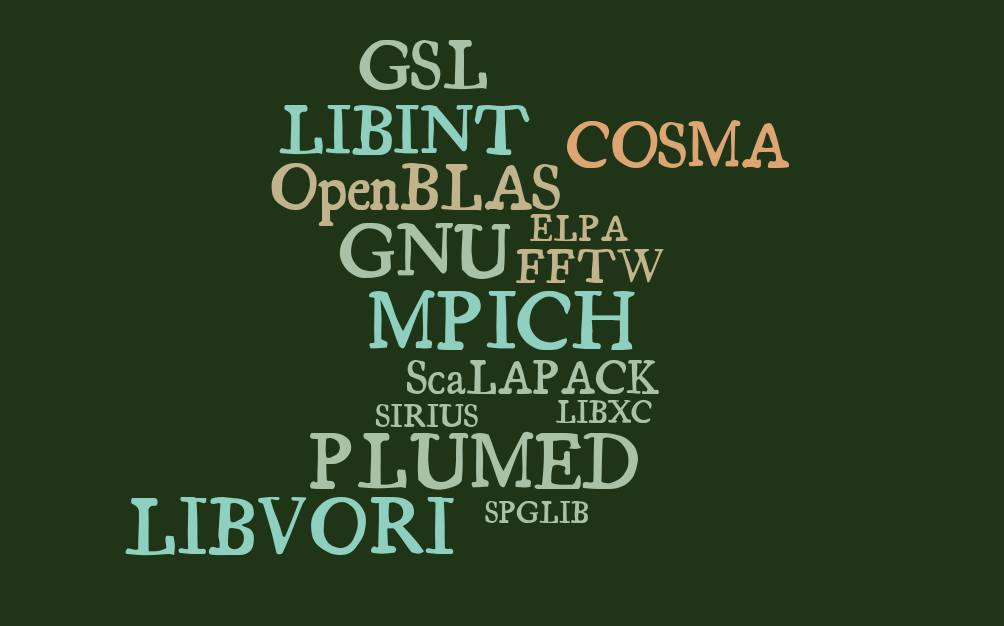
\includegraphics[width=0.7\linewidth]{fig/cp2k-lib.jpg}
    \caption{ไลบรารี่ที่โปรแกรม CP2K ใช้ในการช่วยคำนวณ}
    \label{fig:cp2k_lib}
\end{figure}

ผมจะมาอธิบายบาง Library ที่สำคัญ ๆ ของ CP2K ใช้ ดังนี้

\begin{description}
    \item[GNU] แน่นอนว่าเราต้องคอมไพล์ Source Code ดังนั้นเราจะต้องใช้ตัวคอมไพล์ (Compiler) ซึ่ง CP2K เลือกใช้ GNU เป็น Compiler
    
    \item[OpenBLAS กับ ScaLAPACK]  สำหรับ Linear Algebraic Calculation เช่น Matrix-vector, Matrix-matrix Multiplication 
    
    \item[MPICH] อยากจะรันโปรแกรมแบบขนานโดยใช้ MPI ก็ต้องหา Implementation ที่จะมารันโค้ดของเรา ซึ่ง MPICH ก็เป็นหนึ่งใน
    Implementation ของ MPI ที่ CP2K เลือกใช้
    
    \item[FFTW] สำหรับทำฟูเรียร์ทรานฟอร์มในการคำนวณ DFT หรือแปลงจาก Real Space ไปเป็น Reciprocal Space สำหรับการคำนวณ 
    Electrostatics โดยใช้ Plane Wave Electron Density
    
    \item[LIBXC] เป็น Library ที่ให้เราสามารถนำ DFT Functional มาใช้ได้เลยโดยไม่ต้อง Implement เอง
\end{description}

สรุปก็คือจะเห็นได้ว่าการเขียนโค้ดของโปรแกรมเคมีควอนตัมนั้นมีความซับซ้อนมากดังนั้นเรามีสองทางเลือกคือ 

\begin{enumerate}
    \item ใช้ Library ที่มีอยู่แล้วสำหรับการทำงานเฉพาะจุด
    
    \item เขียนโค้ดทั้งหมดเองเลย
\end{enumerate}

แน่นอนว่าถ้าเราเลือกวิธีแรกก็จะประหยัดเวลาไปได้เยอะมากและเวลาที่เราคอมไพล์โปรแกรมก็ขอแค่ Link กับ Library ต่าง ๆ ก็รันโปรแกรมได้แล้ว%
และทำให้ขนาดของตัวโปรแกรมของเรา (ขนาดของ Binary Files) นั้นมีขนาดไม่ใหญ่มากเกินไปด้วย (เช่นหลักสิบ-ร้อยเมกะไบต์) 

อย่างไรก็ตามโปรแกรมสำหรับจำลองระบบโมเลกุลหลาย ๆ โปรแกรมก็ไม่ได้ใช้ Library เหล่านี้และเลือกใช้วิธีที่ 2 ก็คือการเขียนโค้ดสำหรับการ%
คำนวณส่วนต่าง ๆ เองเลยเนื่องด้วยเหตุหลายข้อ เช่น การเขียนโค้ดทั้งหมดภายใน Framework โปรแกรมเดียวกันนั้นจะทำให้โค้ดมีประสิทธิภาพและ%
ทำงานร่วมกันได้ดี (Compatibility), ง่ายต่อการดูแลรักษาและปรับปรุงโค้ดเพราะว่า Developers นั้นรู้และเข้าใจการทำงานของโค้ดทั้งหมด, 
ถึงแม้ว่าโปรแกรมที่เขียนโค้ดทั้งหมดเองเมื่อถูกคอมไพล์แล้วจะได้ออกมาเป็น Binary File ที่มีขนาดนั้นใหญ่มาก ๆ เช่น หลายกิกะไบต์ แต่ว่าก็มี%
ความคล่องตัวในการใช้งานเพราะว่าไม่ต้องติดตั้ง Library อื่น ๆ เพิ่มเติม 

นอกจากนี้แล้วการที่ใช้ Library หลาย ๆ ตัวแบบนี้ก็มีจุดอ่อนบางข้อที่เราควรจะต้องรู้ไว้นั่นก็คือการเข้ากันได้ (Compatibility) ระหว่าง Library 
หรือเวอร์ชันซึ่งก็อาจจะทำให้เราปวดหัวได้ถ้าหากว่า Library บางตัวมีการอัพเดทเวอร์ชันใหม่แล้ว Conflict กับ Library ตัวอื่น

%----------------------------------------
\section{ทักษะและเครื่องมือสำหรับการเขียนโปรแกรมคำนวณทางวิทยาศาสตร์}
%----------------------------------------

\begin{itemize}
    \item Scripting language: Bash, Python
    
    \item Intensive subroutine with OOP: C++, Fortran
    
    \item Symbolic programming (Mathematica, SymPy)
\end{itemize}

เครื่องมือที่จำเป็น

Tex editor
\begin{itemize}
    \item Vi/Vim, Nano
    
    \item VS Code, Atom, Eclipse, Sublime
\end{itemize}

- File format
  - XML, JSON
  
- General programming skills
  - Type of variables
  - Loops and conditional statement
  - Input/output

- High-level programming
  - Python
    - Pip and conda: Python helper
    - NumPy: Array (vector, matrix) computation
    - Numba: JIT compiler for NumPy
    - Jax: autograd of NumPy array
    - SciPy: a collection of math functions/routines
    - Scikit-learn: statistics routines, optimization, curve fitting
      - Intel Scikit-learn is 10x faster than the standard one
    - Matplotlib / Plotly for plotting graph
    - Theano: numerical computation
    - SCOOP: distributed modules for parallel programming
    - NetworkX: Graph library

- Low-level programming
  - C
    - Function, pointer, storage class
    - Enum, struct, union
    - Preprocessor
    - Operator, memory management, array
    - File handling

  - C++
    - C++ 11 or newer
    - Type of variable: signed, unsigned, long, double, etc.
    - Loops, conditional statement
    - Standard libraries: vector, rand
    - Understanding header (`.hpp`) and source file (`.cpp` or `.cc`)
    - Preprocessor (\texttt{\#if}, \texttt{\#ifdef}, \texttt{\#ifndef}, \texttt{\#define}, etc.)
    - Function, class, struct, template
    - Declaration
      - namespace, const, attribute, pointer, pass by reference, static_assert
    - Initialization
    - Misc: casting, lambda expression, encapsulation, file handling, exception handling

  - Fortran
    - Learn either F77 or F90 or modern fortran (2003, 2008, 2018)
    - Module, subroutine, function
    - Array (allocatable and multidimentional) and string
    - Operator overloading
    - Flow control
    - Derived type
    - Callback
    - Interfacing to other language e.g. Python or C++
  - GNU library
    - GSL
    - Many more libraries [here](https://en.wikipedia.org/wiki/List_of_GNU_packages)

- Memory allocation
  - Stack, heap, global memory

- Math libraries
  - BLAS (OpenBLAS)
  - LAPACK for linear algebra
  - ScaLAPACK - a higher level LAPACK
  - Intel MKL (Intel oneAPI)
  - FFTW: for computing the discrete Fourier transform in one or more dimensions, real and complex data
  - Eigen: linear algebra library
  - Boost: a collection of C++ functions e.g. `regex`, `serialization`

- QM libraries
  - libxc: XC function library
  - libint: For computing Gaussian integral
  - libcint: general GTO integrals

- Code optimization
  - Benchaming/scaling
  - Complexity (Big O)

- GNU
  - Static and dynamic libraries
  - Archive
  - Compiling (g++, gcc) and linking (ld)
  - Useful flags for compiler and linker e.g. `-O2`, `-O3`, `-fPIC`

- Compilng tools
  - autoconf
  - configure
  - Make, cmake, automake

- Debugging
  - gdb for general debugging
  - Valgrind for memory leak analysis

- Git (source code control)
  - Basic/intermediate commands
  - GitHub และ GitLab

- Documentation
  - Sphinx (for markdown and reStructuredText)
  - Doxygen

%----------------------------------------
\section{เขียนโปรแกรม Hartree-Fock SCF ด้วยภาษา Python}
%----------------------------------------

โปรแกรมเคมีควอนตัมทุกโปรแกรมจะต้องมีส่วนหนึ่งของโปรแกรมที่เป็นโค้ดสำหรับแก้สมการอันหนึ่งซึ่งขาดไม่ได้เลยนั่นก็คือ Roothaan-Hall Equation 
โดยใช้วิธี Self-consistent Field ซึ่งเป็นสมการที่เราใช้ในการคำนวณหาพลังงานของระบบที่เราสนใจ

เริ่มต้นสมการ Roothaan-Hall ซึ่งจะเรียกว่าเป็นสมการ HF ที่แปลงร่างมาก็ได้ สาเหตุที่เราต้องแปลงร่าง HF นั่นก็เพราะว่าเราเขียนฟังก์ชันคลื่นใหม่%
ให้อยู่ในรูปที่มี Basis Function (เป็นตัวที่อธิบายออร์บิทัลเชิงอะตอม) นั่นเอง โดยเราจะมีสมการ Roothaan-Hall ทั้งหมด $m$ สมการ โดยที่ $m$ 
คือจำนวนของ Basis Function (เรามีสมการ HF 1 สมการต่อ 1 MO และการที่เรามี m basis function นั้นก็จะสร้างทั้งหมด m MOs ด้วย), 
F คือ Fock matrix ซึ่งก็จะได้จาก Density matrix แล้ว Density matrix ก็คือ matrix ที่มีสมาชิกเป็นผลคูณระหว่าง coefficients ของ 
MO ซึ่งก็จะได้มาจากการประมาณค่าด้วยวิธีเริ่มต้น (initial guess) แบบต่าง ๆ เช่นใช้ Huckel method, ส่วน S นั้นก็คือ Overlap matrix 
ซึ่งก็จะเป็น matrix ที่บอกว่า orbitals นั้นสัมพันธ์กันมากน้อยแค่ไหน, และ epsilon ของแต่ละสมการนั้นก็คือค่าพลังงานของแต่ละ MO 
นั้นเองซึ่งเป็นสิ่งที่เราต้องการแก้สมการหามันออกมา

คราวนี้เราสามารถยุบรวมสมการทั้งหมดในรูปที่ 1 ได้ออกมาเป็นตามสมการที่สั้นและกระชับขึ้นตามรูปที่ 2 ซึ่ง F, C, และ S นั้นเป็น matrix 
ที่มีขนาดคือ m x m แล้วก็ epsilon นั้นก็มีขนาด m x m ด้วย (จะมีเฉพาะสมาชิกในแนวทแยงเท่านั้นที่มีค่าไม่เท่ากับ 0) โดยเราสามารถแสดงสมการด้านซ้ายและขวาให้เป็น matrix ได้ตามรูปที่ 3 และ 4

ประเด็นอยู่ตรงนี้ก็คือตามวิชา linear algebra ถ้าเราต้องการหา matrix ของ epsilon เราสามารถใช้วิธี Diagonalization กับสมการ 
Roothaan-Hall ได้เพราะว่าสมการนี้มันเป็น eigenfunction ซึ่งกระบวนกานที่จะใช้ในการแก้นั้นก็คือตามขั้นตอนต่อไปนี้


กระบวนการ SCF:

เรากำหนดตำแหน่งของอะตอมในโมเลกุล, ประจุ, และทำการเลือก basis seะ

เริ่มคำนวณพลังงานจลน์และพลังงานศักย์ รวมไปถึง overlap integral

คำนวณ orthogonalizing matrix โดยใช้ overlap matrix (overlap matrix ที่ถูกสร้างมาจาก overlap integral ที่ได้จากขั้นที่ 2 อีกที)

คำนวณ Fock matrix อันแรกเลยโดยใช้พลังงานจลน์และพลังงานศักย์แล้วก็ใช้ initial guess ที่ได้จาก coefficients ของ basis set 
ที่กำหนดไว้ตั้งแต่ขั้นตอนที่ 1 โดยหน้าตาของ basis set สามารถดูได้ที่เว็บไซต์ https://www.basissetexchange.org/ ตัวอย่างเช่น 
basis set: aug-cc-PV7Z ของอะตอมคาร์บอน https://www.basissetexchange.org/.../format/nwchem/...

ใช้ orthogonalizing matrix เพื่อแปลงหรือ tranform Fock matrix ให้เป็น matrix อันใหม่ (เรียกว่าเป็น F' ก็แล้วกัน) ที่มันขึ้นอยู่กับ 
orthonal set ของฟังก์ชันที่ได้มาจาก basis set ที่ถูกเซนเตอร์กับอะตอม (atom-centered basis set)

ทำการ diagonalize Fock matrix เพื่อหา coefficient matrix ที่ถูก transform มาแล้ว (เรียกว่า C') ก็ได้แล้วก็หาพลังงานของแต่ละ MO ได้

เปรียบเทียบ C' และพลังงานกับค่าที่ได้จากรอบก่อนหน้านี้ ถ้าผลต่างยังไม่น้อยกว่า cutoff ที่กำหนดไว้ก็ให้นำ Fock matrix ที่ได้มาล่าสุดไปใช้ใหม่อีกครั้งหนึ่งในขั้นที่ 4 ทำวนไปเรื่อย ๆ จนได้คำตอบที่แม่นยำ

%----------------------------------------
\section{เขียนโปรแกรม MP2 ด้วยภาษา Python}
%----------------------------------------

%----------------------------------------
\section{เขียนโปรแกรม DFT ด้วยภาษา Python}
%----------------------------------------

%----------------------------------------
\subsection{เขียนโปรแกรมสำหรับคำนวณ Kohn-Sham Matrix}
%----------------------------------------

%----------------------------------------
\subsection{เขียนโปรแกรมฟังก์ชันนอล LDA}
%----------------------------------------

%----------------------------------------
\subsection{เขียนโปรแกรมฟังก์ชันนอล B3LYP}
%----------------------------------------

%----------------------------------------
\section{แบบฝึกหัด}
%----------------------------------------
